\documentclass[10pt]{article}

\usepackage[margin=0.72in]{geometry}
\usepackage{booktabs}
\usepackage{array}
\usepackage{longtable}
\usepackage{tabularx}
\usepackage{graphicx}
\usepackage{xcolor}
\usepackage{float}
\usepackage[hidelinks]{hyperref}
\usepackage{microtype}

\setlength{\emergencystretch}{2em}
\setlength{\parindent}{0pt}
\setlength{\parskip}{0.45em}
\renewcommand{\thetable}{S\arabic{table}}
\renewcommand{\thefigure}{S\arabic{figure}}

\title{Supplementary Material for\\
MOSAIC: branch-supervised CITE-seq annotation with auditable modality evidence under donor shift and incomplete protein panels}
\author{Hai Yang, Linhao Wu, Dan Zhou, Tianyi Zhou, Qin Zhou,\\
Ting Xiao, Qian Zhang, Jing Zhang, and Zhe Wang}
\date{23 July 2026}

\begin{document}
\maketitle

\section{Evidence policy}

The primary statistical protocol is nested leave-one-donor-out evaluation. Test donor, validation donor and six training donors are disjoint. Gene selection and RNA/ADT transformations are fitted using training donors only. Three model seeds are averaged within each held-out donor, and the eight donors are the biological replicates. Cell counts and seeds are not treated as independent biological observations.

The supplement distinguishes four evidence types: retrained method comparisons, same-checkpoint inference ablations, deterministic missing-panel stress tests and constructed leave-class-out stress tests. PDC101 uses a separate label space and protocol, so it is reported as a compatible direct hierarchy comparison rather than pooled with PBMC. Older random-cell, COVID-19, 5P and COMBAT results are retained as secondary breadth evidence and do not replace the donor-disjoint inference.

\section{Dataset lineage and nested splits}

The GSE164378 3P and 5P cohorts contain the same eight donors and are not independent-donor datasets. The primary 3P source contains 161,764 cells, 58 L3 labels and 224 proteins. For each fold, 3,000 genes are selected using the six training donors. Every training fold contains all 58 labels, so natural held-out-donor evaluation is closed set.

\begin{table}[H]
\centering
\caption{Nested donor split sizes. Validation donors follow a fixed cycle; no donor occurs in more than one partition within a fold.}
\label{tab:splits}
\small
\begin{tabular}{lrrrr}
\toprule
Test donor & Validation donor & Training cells & Validation cells & Test cells \\
\midrule
P1 & P2 & 126,424 & 17,205 & 18,135 \\
P2 & P3 & 129,899 & 14,660 & 17,205 \\
P3 & P4 & 130,014 & 17,090 & 14,660 \\
P4 & P5 & 122,863 & 21,811 & 17,090 \\
P5 & P6 & 119,211 & 20,742 & 21,811 \\
P6 & P7 & 115,151 & 25,871 & 20,742 \\
P7 & P8 & 109,643 & 26,250 & 25,871 \\
P8 & P1 & 117,379 & 18,135 & 26,250 \\
\bottomrule
\end{tabular}
\end{table}

Split manifests are stored under
\texttt{configs/splits/pbmc\_cite\_seq/nested\_lodo/}. The aggregate cache audit is
\texttt{results/tables/mosaic\_n\_v33\_nested\_lodo\_cache\_summary\_2026-07-23.csv}.
Each cache records label support and confirms that feature selection and scalers were fitted on training donors only.

\section{Complete nested-donor performance matrix}

Table~\ref{tab:donor-full} reports retrained methods and same-checkpoint inference variants. The point estimate for each donor is the mean of seeds 41, 42 and 43. The 95\% interval is then calculated across eight donor means. ``Worst donor'' is the minimum score for performance metrics.

\begin{table}[H]
\centering
\caption{Complete nested donor-disjoint performance matrix.}
\label{tab:donor-full}
\scriptsize
\setlength{\tabcolsep}{2.8pt}
\resizebox{\textwidth}{!}{%
\begin{tabular}{llccc}
\toprule
Method & Metric & Mean [95\% CI] & Worst donor & $n$ donors \\
\midrule
ADT branch & accuracy & 0.8360 [0.8245, 0.8474] & 0.8149 & 8 \\
ADT branch & weighted\_f1 & 0.8364 [0.8270, 0.8457] & 0.8159 & 8 \\
ADT branch & macro\_f1 & 0.6661 [0.6515, 0.6808] & 0.6360 & 8 \\
Fusion branch & accuracy & 0.9100 [0.9070, 0.9130] & 0.9042 & 8 \\
Fusion branch & weighted\_f1 & 0.9092 [0.9052, 0.9133] & 0.9005 & 8 \\
Fusion branch & macro\_f1 & 0.8059 [0.7919, 0.8198] & 0.7771 & 8 \\
Learned margin gate & accuracy & 0.9119 [0.9086, 0.9153] & 0.9055 & 8 \\
Learned margin gate & weighted\_f1 & 0.9107 [0.9062, 0.9153] & 0.9010 & 8 \\
Learned margin gate & macro\_f1 & 0.8077 [0.7925, 0.8228] & 0.7794 & 8 \\
Learned margin gate + HSR & accuracy & 0.9119 [0.9086, 0.9153] & 0.9057 & 8 \\
Learned margin gate + HSR & weighted\_f1 & 0.9108 [0.9062, 0.9153] & 0.9012 & 8 \\
Learned margin gate + HSR & macro\_f1 & 0.8072 [0.7917, 0.8227] & 0.7792 & 8 \\
RNA branch & accuracy & 0.8894 [0.8846, 0.8942] & 0.8827 & 8 \\
RNA branch & weighted\_f1 & 0.8882 [0.8825, 0.8940] & 0.8805 & 8 \\
RNA branch & macro\_f1 & 0.7564 [0.7402, 0.7726] & 0.7293 & 8 \\
Uniform fusion & accuracy & 0.9130 [0.9096, 0.9164] & 0.9068 & 8 \\
Uniform fusion & weighted\_f1 & 0.9118 [0.9072, 0.9165] & 0.9021 & 8 \\
Uniform fusion & macro\_f1 & 0.8114 [0.7961, 0.8266] & 0.7803 & 8 \\
MLP early fusion & accuracy & 0.9091 [0.9048, 0.9133] & 0.9023 & 8 \\
MLP early fusion & weighted\_f1 & 0.9068 [0.9020, 0.9116] & 0.8987 & 8 \\
MLP early fusion & macro\_f1 & 0.7923 [0.7758, 0.8089] & 0.7626 & 8 \\
MOSAIC full & accuracy & 0.9119 [0.9086, 0.9153] & 0.9057 & 8 \\
MOSAIC full & weighted\_f1 & 0.9108 [0.9062, 0.9153] & 0.9012 & 8 \\
MOSAIC full & macro\_f1 & 0.8072 [0.7917, 0.8227] & 0.7792 & 8 \\
MOSAIC without HSR & accuracy & 0.9135 [0.9102, 0.9168] & 0.9081 & 8 \\
MOSAIC without HSR & weighted\_f1 & 0.9121 [0.9079, 0.9162] & 0.9057 & 8 \\
MOSAIC without HSR & macro\_f1 & 0.8097 [0.7950, 0.8243] & 0.7847 & 8 \\
MOSAIC without KD & accuracy & 0.9134 [0.9102, 0.9167] & 0.9092 & 8 \\
MOSAIC without KD & weighted\_f1 & 0.9121 [0.9078, 0.9164] & 0.9049 & 8 \\
MOSAIC without KD & macro\_f1 & 0.8110 [0.7956, 0.8265] & 0.7813 & 8 \\
\bottomrule
\end{tabular}

}
\end{table}

MOSAIC full versus MLP produced paired differences of $+0.0029$ ACC (95\% CI $-0.0001$ to 0.0059; paired $P=0.0588$), $+0.0040$ W-F1 (0.0013--0.0066; $P=0.0101$) and $+0.0148$ M-F1 (0.0091--0.0206; $P=0.0005$). Wilcoxon sensitivity $P$ values were 0.0547, 0.0156 and 0.0078, respectively. These unadjusted tests describe three prespecified aggregate metrics and are not generalized to every exploratory per-class comparison.

The direct architecture ablations were unfavorable to the full configuration. Full minus no-HSR was $-0.0016$ ACC, $-0.0013$ W-F1 and $-0.0025$ M-F1. Full minus no-KD was $-0.0015$, $-0.0014$ and $-0.0038$. Same-checkpoint learned margin gate plus HSR minus uniform fusion was $-0.0011$ ACC, $-0.0011$ W-F1 and $-0.0042$ M-F1, with all eight donor differences negative. The full paired table is
\texttt{results/tables/mosaic\_n\_v33\_paired\_donor\_statistics\_2026-07-23.csv}.

Per-class results exclude donor--class combinations with zero true support rather than assigning F1 zero. The support-aware table is
\texttt{results/tables/mosaic\_n\_v33\_donor\_per\_class\_summary\_2026-07-23.csv}.
Predictions into a class absent from a donor's truth set remain penalized in donor-level aggregate metrics.

\section{Branch and auditability closure}

The branch-supervision sensitivity matrix used the same nested leave-one-donor-out protocol as the primary table. It reused the same train-only caches, validation-donor mapping, seed set and teacher-probability protocol. The tested configurations were $\lambda_b=0$, $\lambda_b=0.15$, $\lambda_b=0.70$ and a late-fusion-only setting with $\lambda_b=0,\lambda_f=1$. The primary full configuration corresponds to $\lambda_b=0.35,\lambda_f=0.5$ and is reported in Table~\ref{tab:donor-full}.

\begin{table}[H]
\centering
\caption{Branch-supervision sensitivity under the primary nested donor protocol. Values are donor means with 95\% confidence intervals after averaging three seeds within each donor.}
\label{tab:branch-supervision}
\scriptsize
\setlength{\tabcolsep}{2.8pt}
\resizebox{\textwidth}{!}{%
\begin{tabular}{lccccc}
\toprule
Metric & $\lambda_b=0,\lambda_f=0.5$ & $\lambda_b=0.15,\lambda_f=0.5$ & locked $\lambda_b=0.35,\lambda_f=0.5$ & $\lambda_b=0.70,\lambda_f=0.5$ & fusion-only $\lambda_b=0,\lambda_f=1$ \\
\midrule
ACC & 0.9102 [0.9065, 0.9139] & 0.9103 [0.9068, 0.9138] & 0.9119 [0.9086, 0.9153] & \textbf{0.9140 [0.9111, 0.9169]} & 0.9108 [0.9075, 0.9142] \\
W-F1 & 0.9095 [0.9052, 0.9137] & 0.9094 [0.9053, 0.9135] & 0.9108 [0.9062, 0.9153] & \textbf{0.9126 [0.9086, 0.9165]} & 0.9099 [0.9055, 0.9143] \\
M-F1 & 0.8084 [0.7937, 0.8230] & 0.8061 [0.7924, 0.8199] & 0.8072 [0.7917, 0.8227] & 0.8092 [0.7920, 0.8264] & \textbf{0.8122 [0.7992, 0.8251]} \\
Balanced ACC & 0.8097 [0.7922, 0.8272] & 0.8082 [0.7954, 0.8210] & \textbf{0.8085 [0.7890, 0.8280]} & 0.8063 [0.7863, 0.8264] & 0.8132 [0.7989, 0.8276] \\
\bottomrule
\end{tabular}

}
\end{table}

The sensitivity curve does not support a monotonic ``more branch supervision is always better'' claim. $\lambda_b=0.70$ produced the highest ACC and W-F1, while late-fusion-only training produced the highest M-F1 and balanced accuracy. We therefore interpret branch supervision as an architecture and auditability choice with measurable metric trade-offs, not as a single universally positive module.

\begin{table}[H]
\centering
\caption{Quantitative auditability closure. Branch-disagreement and uncertainty scores use final prediction error as the target. HSR action rates are averaged over full checkpoints. Attribution faithfulness reports top-feature deletion lift over matched random deletion.}
\label{tab:auditability-closure}
\scriptsize
\setlength{\tabcolsep}{3pt}
\resizebox{\textwidth}{!}{%
\begin{tabular}{llc}
\toprule
Audit question & Measurement & Donor-level result \\
\midrule
Branch disagreement & error AUROC & 0.7552 [0.7445, 0.7659] \\
Branch disagreement & error AUPRC & 0.2394 [0.2277, 0.2511] \\
Branch disagreement & risk at 90\% coverage & 0.0637 [0.0605, 0.0669] \\
Final uncertainty & error AUROC & 0.6914 [0.6507, 0.7320] \\
Final uncertainty & error AUPRC & 0.3100 [0.2906, 0.3294] \\
Final uncertainty & risk at 90\% coverage & 0.0563 [0.0513, 0.0614] \\
HSR action audit & HSR prediction-change rate & 0.0015 [0.0010, 0.0020] \\
HSR action audit & HSR wrong-to-correct rate & 0.0006 [0.0005, 0.0008] \\
HSR action audit & HSR correct-to-wrong rate & 0.0006 [0.0004, 0.0008] \\
Attribution faithfulness & ADT top-feature deletion lift & 0.2358; positive 6/6 tests \\
Attribution faithfulness & RNA top-feature deletion lift & 0.1304; positive 6/6 tests \\
\bottomrule
\end{tabular}

}
\end{table}

Branch disagreement improved error-detection AUROC over final uncertainty but did not dominate uncertainty in AUPRC or risk at 90\% coverage. This makes it useful as a complementary diagnostic for modality conflict. HSR changed only 0.0015 of predictions on average; wrong-to-correct and correct-to-wrong changes were balanced. Same-checkpoint TOST equivalence within $\delta=0.005$ was supported for HSR across ACC, W-F1, M-F1 and balanced accuracy. Retrained KD and HSR comparisons were metric-dependent and should not be summarized as uniformly equivalent.

\begin{table}[H]
\centering
\caption{Branch margin-correctness audit. Top-two logit margins were computed separately for RNA, ADT and fusion branches in each donor--seed checkpoint. Spearman correlations and quintile summaries use held-out donor as the statistical unit after averaging seeds.}
\label{tab:margin-correctness}
\scriptsize
\setlength{\tabcolsep}{3pt}
\resizebox{\textwidth}{!}{%
\begin{tabular}{lrrrrrr}
\toprule
Branch & Accuracy & Spearman & Top--bottom accuracy & Monotonic steps & Median margin (IQR) & $\beta$ \\
\midrule
ADT & 0.836 [0.824, 0.847] & 0.456 [0.445, 0.468] & 0.467 [0.452, 0.481] & 3.96 [3.86, 4.00] & 2.666 [1.156, 3.730] & -0.501 \\
Fusion & 0.910 [0.907, 0.913] & 0.289 [0.254, 0.324] & 0.273 [0.250, 0.297] & 2.46 [1.94, 2.97] & 4.467 [3.768, 5.062] & +0.632 \\
RNA & 0.889 [0.885, 0.894] & 0.388 [0.378, 0.397] & 0.372 [0.359, 0.384] & 3.62 [3.39, 3.86] & 3.496 [2.312, 4.251] & -0.035 \\
Mean over branches & 0.878 [0.874, 0.883] & 0.378 [0.365, 0.390] & 0.370 [0.364, 0.377] & 3.35 [3.11, 3.59] & 3.543 [2.412, 4.348] & +0.032 \\
\bottomrule
\end{tabular}

}
\end{table}

The branch margin audit supports the use of branch margins as a confidence-like diagnostic. All three branches had positive donor-level Spearman correlations between top-two logit margin and branch correctness. The effect was strongest for ADT and RNA and weaker for fusion, consistent with the fusion branch already operating at higher baseline accuracy. This result validates margin as an ordering signal; it does not imply that margin gating alone improves every aggregate metric.

\section{Missing-protein and panel-mismatch stress tests}

Twenty-four full checkpoints were evaluated under eight deterministic conditions without retraining or test-label policy selection. Random masks remove the same fixed feature subset for all cells within a fold/seed condition. Marker masks remove six memory-associated or 15 T-cell-associated ADTs after alias normalization.

\begin{table}[H]
\centering
\caption{Frozen-checkpoint performance and calibration under protein-panel masks. Intervals use held-out donor after averaging seeds. For ECE, the worst donor is the maximum value.}
\label{tab:panel}
\scriptsize
\setlength{\tabcolsep}{2.8pt}
\resizebox{\textwidth}{!}{%
\begin{tabular}{llcccccc}
\toprule
Scenario & Metric & Removed ADTs & Removed fraction & Mean [95\% CI] & $\Delta$M-F1 / fraction & Worst donor & $n$ donors/units \\
\midrule
full & weighted\_f1 & 0 & 0.0\% & 0.9108 [0.9062, 0.9153] & -- & 0.9012 & 8 \\
full & macro\_f1 & 0 & 0.0\% & 0.8072 [0.7917, 0.8227] & 0.0000 & 0.7792 & 8 \\
full & ece & 0 & 0.0\% & 0.0713 [0.0645, 0.0781] & -- & 0.0874 & 8 \\
full & Brier & 0 & 0.0\% & 0.1523 [0.1456, 0.1591] & -- & 0.1629 & 8 \\
full\_val\_temperature & ece & 0 & 0.0\% & 0.0391 [0.0303, 0.0478] & -- & 0.0527 & 8 \\
full\_val\_temperature & Brier & 0 & 0.0\% & 0.1462 [0.1380, 0.1545] & -- & 0.1588 & 8 \\
marker\_memory & weighted\_f1 & 6 & 2.7\% & 0.9082 [0.9038, 0.9126] & -- & 0.8991 & 8 \\
marker\_memory & macro\_f1 & 6 & 2.7\% & 0.8006 [0.7833, 0.8180] & 0.2464 & 0.7678 & 8 \\
marker\_memory & ece & 6 & 2.7\% & 0.0738 [0.0670, 0.0806] & -- & 0.0899 & 8 \\
marker\_memory & Brier & 6 & 2.7\% & 0.1564 [0.1495, 0.1634] & -- & 0.1674 & 8 \\
marker\_tcell & weighted\_f1 & 15 & 6.7\% & 0.9021 [0.8969, 0.9072] & -- & 0.8950 & 8 \\
marker\_tcell & macro\_f1 & 15 & 6.7\% & 0.7859 [0.7709, 0.8008] & 0.3180 & 0.7647 & 8 \\
marker\_tcell & ece & 15 & 6.7\% & 0.0748 [0.0664, 0.0832] & -- & 0.0934 & 8 \\
marker\_tcell & Brier & 15 & 6.7\% & 0.1661 [0.1591, 0.1731] & -- & 0.1753 & 8 \\
\multicolumn{8}{l}{\emph{V8.2 size-matched random-null rows; intervals use 24 frozen donor--seed units and worst donor is not estimable.}} \\
random\_size\_matched\_6 & weighted\_f1 & 6 & 2.7\% & 0.9103 [0.9079, 0.9126] & -- & -- & 24 units \\
random\_size\_matched\_6 & macro\_f1 & 6 & 2.7\% & 0.8070 [0.7998, 0.8143] & 0.0059 & -- & 24 units \\
random\_size\_matched\_15 & weighted\_f1 & 15 & 6.7\% & 0.9089 [0.9066, 0.9112] & -- & -- & 24 units \\
random\_size\_matched\_15 & macro\_f1 & 15 & 6.7\% & 0.8028 [0.7943, 0.8113] & 0.0658 & -- & 24 units \\
random\_10 & weighted\_f1 & 22 & 10.0\% & 0.9074 [0.9015, 0.9132] & -- & 0.8957 & 8 \\
random\_10 & macro\_f1 & 22 & 10.0\% & 0.8003 [0.7824, 0.8182] & 0.0702 & 0.7702 & 8 \\
random\_10 & ece & 22 & 10.0\% & 0.0728 [0.0662, 0.0795] & -- & 0.0892 & 8 \\
random\_10 & Brier & 22 & 10.0\% & 0.1572 [0.1487, 0.1658] & -- & 0.1704 & 8 \\
random\_30 & weighted\_f1 & 67 & 30.0\% & 0.9020 [0.8963, 0.9076] & -- & 0.8920 & 8 \\
random\_30 & macro\_f1 & 67 & 30.0\% & 0.7904 [0.7742, 0.8066] & 0.0562 & 0.7634 & 8 \\
random\_30 & ece & 67 & 30.0\% & 0.0755 [0.0682, 0.0827] & -- & 0.0924 & 8 \\
random\_30 & Brier & 67 & 30.0\% & 0.1661 [0.1578, 0.1745] & -- & 0.1787 & 8 \\
random\_50 & weighted\_f1 & 112 & 50.0\% & 0.8971 [0.8903, 0.9039] & -- & 0.8830 & 8 \\
random\_50 & macro\_f1 & 112 & 50.0\% & 0.7742 [0.7557, 0.7927] & 0.0660 & 0.7424 & 8 \\
random\_50 & ece & 112 & 50.0\% & 0.0764 [0.0669, 0.0859] & -- & 0.0985 & 8 \\
random\_50 & Brier & 112 & 50.0\% & 0.1741 [0.1647, 0.1835] & -- & 0.1904 & 8 \\
random\_70 & weighted\_f1 & 157 & 70.0\% & 0.8921 [0.8855, 0.8988] & -- & 0.8813 & 8 \\
random\_70 & macro\_f1 & 157 & 70.0\% & 0.7641 [0.7453, 0.7829] & 0.0615 & 0.7337 & 8 \\
random\_70 & ece & 157 & 70.0\% & 0.0770 [0.0680, 0.0859] & -- & 0.0965 & 8 \\
random\_70 & Brier & 157 & 70.0\% & 0.1811 [0.1706, 0.1915] & -- & 0.1954 & 8 \\
rna\_only & weighted\_f1 & 224 & 100.0\% & 0.8882 [0.8826, 0.8938] & -- & 0.8810 & 8 \\
rna\_only & macro\_f1 & 224 & 100.0\% & 0.7558 [0.7390, 0.7726] & 0.0514 & 0.7306 & 8 \\
rna\_only & ece & 224 & 100.0\% & 0.1063 [0.0914, 0.1212] & -- & 0.1330 & 8 \\
rna\_only & Brier & 224 & 100.0\% & 0.1888 [0.1826, 0.1950] & -- & 0.2036 & 8 \\
\bottomrule
\end{tabular}

}
\end{table}

The donor-level W-F1 degradation slope over 0/10/30/50/70\% random masking was $-0.0263\pm0.0071$ per fully missing protein fraction. The M-F1 slope was $-0.0624\pm0.0108$. Brier score increased by $0.0411\pm0.0097$ per full missing fraction. ECE slope was less stable ($+0.0081\pm0.0072$), whereas the RNA-only ECE increase was clear. These are post hoc robustness measurements of a full-input model, not evidence that the model was trained for arbitrary missing modalities.

\section{Leave-class-out rejection and hierarchy fallback}

The five target labels were removed from all training and validation labels before each 57-class model was fitted. Unknown test cells retained the removed label only for evaluation. Thresholds were selected from known validation scores at target known coverage 0.95 or 0.80. No unknown validation or test label informed the threshold.

\begin{table}[H]
\centering
\caption{Aggregate validation-selected rejection results. Values first average three seeds within each target and then average five leave-class-out targets.}
\label{tab:unknown-aggregate}
\scriptsize
\setlength{\tabcolsep}{2.5pt}
\resizebox{\textwidth}{!}{%
\input{tables/v33/supplement_unknown_reject.tex}
}
\end{table}

\begin{table}[H]
\centering
\caption{Per-target margin-score results at target known coverage 0.80. Support and target difficulty vary substantially.}
\label{tab:unknown-target}
\scriptsize
\setlength{\tabcolsep}{3pt}
\resizebox{\textwidth}{!}{%
\begin{tabular}{lrrrrrrr}
\toprule
Target & $n$ unknown & Known coverage & Unknown recall & AUROC & Parent-safe rate & Hierarchical accuracy & Panel marker \\
\midrule
B naive lambda & 83 & 0.7927 & 0.1285 & 0.4258 & 0.0723 & 0.9277 & N: kappa/lambda \\
CD4 TCM\_1 & 734 & 0.7807 & 0.5722 & 0.7284 & 0.2489 & 0.9167 & Y: CD4/RO/27 \\
CD8 TEM\_4 & 1291 & 0.7897 & 0.4056 & 0.5696 & 0.3945 & 0.9011 & Y: CD8/RO/27 \\
NK\_3 & 614 & 0.7847 & 0.3458 & 0.5474 & 0.3371 & 0.9192 & Y: CD56/335 \\
gdT\_2 & 583 & 0.7914 & 0.5638 & 0.7026 & 0.0766 & 0.9083 & Y: TCR-V \\
\bottomrule
\end{tabular}

}
\end{table}

B naive lambda is the smallest unknown set ($n=83$) and produced below-chance AUROC and low recall. CD4 TCM\_1 and gdT\_2 were easier to rank as unknown, but gdT\_2 had low parent-safe fallback. The mean unknown parent-safe rate at the chosen margin operating point was only 0.2259. These results preclude a broad open-set or safe-hierarchy claim.

\begin{table}[H]
\centering
\caption{Light-chain feature availability for interpreting the B naive lambda leave-class-out failure. RNA markers are checked after each train-only 3,000-gene selection. ADT reports whether a kappa/lambda-like surface marker is present in the 224-protein panel.}
\label{tab:light-chain}
\small
\begin{tabular}{lcc}
\toprule
Feature & Type & Present donors \\
\midrule
kappa\_or\_lambda\_surface\_marker & ADT & 0/8 \\
IGKC & RNA & 8/8 \\
IGLC1 & RNA & 0/8 \\
IGLC2 & RNA & 8/8 \\
IGLC3 & RNA & 8/8 \\
IGLC4 & RNA & 0/8 \\
IGLC5 & RNA & 0/8 \\
IGLC6 & RNA & 0/8 \\
IGLC7 & RNA & 0/8 \\
\bottomrule
\end{tabular}

\end{table}

IGKC, IGLC2 and IGLC3 were retained in every donor fold, whereas IGLC1 and IGLC4--7 were not retained. The ADT panel did not contain a kappa/lambda surface marker. This supports a concrete interpretation for the B naive lambda pseudo-unknown failure: the class boundary is light-chain specific, and the multimodal input lacks a directly matched protein marker.

\section{PDC101 comparison with official MMoCHi}

PDC101 preprocessing was audited before the final comparison. The h5ad RNA matrix was already log-transformed and the protein matrix was already processed; an initial runner that repeated log and quantile transformations was invalidated and archived separately. The valid runner uses the processed matrices, fits only StandardScaler on training cells, excludes HTO/isotype/control proteins and validates every official external-holdout identifier and truth label.

\begin{table}[H]
\centering
\caption{PDC101 same-holdout aggregate comparison. Uncertainty modes are not interchangeable.}
\label{tab:pdc-aggregate}
\small
\resizebox{\textwidth}{!}{%
\begin{tabular}{llcc}
\toprule
Method & Metric & Mean [95\% CI] & Mode \\
\midrule
MOSAIC & accuracy & 0.9077 [0.8897, 0.9257] & seed Student-t \\
MOSAIC & weighted\_f1 & 0.9068 [0.8881, 0.9255] & seed Student-t \\
MOSAIC & macro\_f1 & 0.9007 [0.8798, 0.9216] & seed Student-t \\
MMoCHi & accuracy & 0.9347 [0.9237, 0.9457] & cell bootstrap; conditional on one workflow \\
MMoCHi & weighted\_f1 & 0.9335 [0.9221, 0.9449] & cell bootstrap; conditional on one workflow \\
MMoCHi & macro\_f1 & 0.9298 [0.9180, 0.9416] & cell bootstrap; conditional on one workflow \\
\bottomrule
\end{tabular}

}
\end{table}

\begin{table}[H]
\centering
\caption{PDC101 per-class F1 point estimates on the 2,098-cell sorted holdout.}
\label{tab:pdc-class}
\small
\begin{tabular}{lrrrr}
\toprule
Class & Support & MOSAIC F1 & MMoCHi F1 & $\Delta$ F1 (MOSAIC--MMoCHi) \\
\midrule
cd8\_emra & 206 & 0.8863 & 0.9493 & -0.0630 \\
cd8\_cm & 223 & 0.8246 & 0.8851 & -0.0605 \\
cd8\_n & 241 & 0.9260 & 0.9734 & -0.0474 \\
cd8\_em & 365 & 0.8825 & 0.9122 & -0.0297 \\
cd4\_cm & 207 & 0.8185 & 0.8435 & -0.0250 \\
cd4\_em & 295 & 0.9374 & 0.9420 & -0.0046 \\
cd4\_n & 227 & 0.9333 & 0.9358 & -0.0025 \\
monocyte & 334 & 0.9970 & 0.9970 & +0.0000 \\
\bottomrule
\end{tabular}

\end{table}

MMoCHi exceeded MOSAIC for every aggregate metric and most classes. The largest gaps occurred at CD8 central-memory/effector-memory boundaries. Monocyte F1 was identical. MMoCHi intervals are cell bootstrap intervals conditional on one official workflow fit; MOSAIC intervals are Student-$t$ margins over three model seeds.

\begin{figure}[H]
\centering
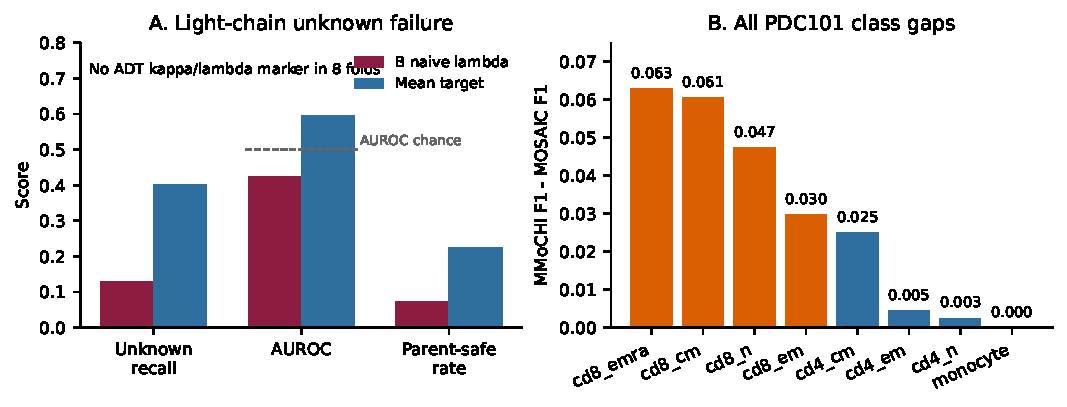
\includegraphics[width=\textwidth]{Fig/FigS_case_study_marker_limits.pdf}
\caption{Case-study evidence for marker-limited behavior. (a) B naive lambda was the hardest leave-class-out target, with low unknown recall, below-chance AUROC and low parent-safe rate; the ADT panel contained no kappa/lambda-like marker in any donor fold. (b) On PDC101, the largest MMoCHi--MOSAIC F1 gaps were concentrated in CD8 memory/effector-memory-related classes, whereas monocyte F1 was identical.}
\label{fig:case-study}
\end{figure}

These two cases show different limits of the current model. B naive lambda illustrates absent marker evidence for unknown detection, whereas the PDC101 CD8 boundary illustrates a setting where an official curated hierarchy better matches the label structure than a learned high-dimensional reference classifier.

\section{Computational cost}

Runtime summaries were rebuilt from the primary nested-donor \texttt{results\_summary.csv} artifacts. Each run corresponds to one held-out donor and one seed. Parameter counts use the primary configuration dimensions: 3,000 RNA genes, 224 ADTs, 58 classes, MLP hidden dimensions 512/128, and MOSAIC hidden dimension 256 with branch encoders, fusion encoder and linear L3 heads. Runtime does not include raw-data download or public release packaging.

\begin{table}[H]
\centering
\caption{Computational cost in the primary nested donor matrix. Runtime is wall-clock training time per fold--seed unit recorded in the run summaries.}
\label{tab:computational-cost}
\small
\resizebox{\textwidth}{!}{%
\begin{tabular}{lrrrrc}
\toprule
Method & Parameters & Runs & Median runtime (s) & Runtime range (s) & Device \\
\midrule
MLP early fusion & 1.73M & 24 & 62.3 & 48.1--88.8 & cuda \\
MOSAIC full & 2.51M & 24 & 130.0 & 89.5--201.1 & cuda \\
MOSAIC without HSR & 2.42M & 24 & 146.0 & 82.6--179.4 & cuda \\
MOSAIC without KD & 2.51M & 24 & 135.9 & 89.7--182.3 & cuda \\
\bottomrule
\end{tabular}

}
\end{table}

\section{Full-training published and strong ML donor baselines}

To expand baseline coverage without an asymmetric training-cap caveat, we reran one published single-cell annotation package baseline and 12 classical or tree-based baselines on the primary nested donor protocol using all cells from the six training donors in each fold. Each method was evaluated on the complete held-out donor, and no validation or test label was used for model selection. CellTypist was run as an RNA-only published-method baseline on the train-only standardized RNA tensors. XGBoost, nearest-centroid and Gaussian naive Bayes variants were run separately for RNA-only, ADT-only and early-fusion RNA+ADT inputs; ridge baselines were rerun with the same uncapped training protocol. The displayed ranking table excludes Gaussian naive Bayes because the high-dimensional likelihood model produced clearly unstable rows; those diagnostic runs remain in the raw artifacts but are not used as ranking comparators.

R/Bioconductor scmap and scPred reproductions remain available as additional tool-coverage artifacts, but are not included in Table~\ref{tab:strong-ml-baselines} because their local runs used method-specific caps for tractability. Thus, Table~\ref{tab:strong-ml-baselines} is the uncapped strong-baseline matrix used for the main comparator caveat closure.

\begin{table}[H]
\centering
\caption{Full-training published and strong ML baselines under the primary PBMC donor-disjoint L3 protocol. Values are donor means with 95\% confidence intervals across eight held-out donors. All listed baselines use the full six training donors in each fold and the complete held-out donor test set. Diagnostic Gaussian naive Bayes runs are excluded from this ranking table.}
\label{tab:strong-ml-baselines}
\scriptsize
\setlength{\tabcolsep}{2.6pt}
\resizebox{\textwidth}{!}{%
\begin{tabular}{llrrrrrr}
\toprule
Method & Modality & ACC & W-F1 & M-F1 & B-ACC & Worst ACC & Best ACC \\
\midrule
CellTypist-compatible subset-first & RNA-only & 0.8652 [0.8573, 0.8732] & 0.8565 [0.8477, 0.8654] & 0.6559 [0.6249, 0.6870] & 0.6240 [0.5950, 0.6530] & 0.8486 & 0.8767 \\
CellTypist-compatible full-denominator & RNA-only & 0.8534 [0.8391, 0.8677] & 0.8497 [0.8350, 0.8644] & 0.6835 [0.6608, 0.7062] & 0.6933 [0.6731, 0.7136] & 0.8310 & 0.8712 \\
Early-fusion XGBoost (uncapped) & RNA+ADT & 0.9032 [0.8912, 0.9152] & 0.9010 [0.8901, 0.9120] & 0.7885 [0.7648, 0.8122] & 0.7755 [0.7543, 0.7968] & 0.8750 & 0.9201 \\
RNA XGBoost (uncapped) & RNA-only & 0.8741 [0.8637, 0.8846] & 0.8681 [0.8566, 0.8796] & 0.7168 [0.6969, 0.7368] & 0.6967 [0.6743, 0.7192] & 0.8474 & 0.8979 \\
ADT XGBoost (uncapped) & ADT-only & 0.8426 [0.8313, 0.8540] & 0.8349 [0.8254, 0.8444] & 0.6557 [0.6371, 0.6742] & 0.6429 [0.6273, 0.6584] & 0.8185 & 0.8679 \\
Early-fusion ridge & RNA+ADT & 0.8547 [0.8442, 0.8652] & 0.8571 [0.8471, 0.8672] & 0.7028 [0.6814, 0.7242] & 0.7660 [0.7556, 0.7763] & 0.8349 & 0.8720 \\
RNA ridge & RNA-only & 0.8329 [0.8179, 0.8479] & 0.8373 [0.8245, 0.8500] & 0.6706 [0.6486, 0.6925] & 0.7412 [0.7303, 0.7520] & 0.8067 & 0.8587 \\
ADT ridge & ADT-only & 0.7595 [0.7411, 0.7778] & 0.7626 [0.7448, 0.7803] & 0.5072 [0.4819, 0.5326] & 0.6460 [0.6280, 0.6640] & 0.7299 & 0.7952 \\
Early-fusion centroid & RNA+ADT & 0.7244 [0.6581, 0.7907] & 0.7395 [0.6826, 0.7963] & 0.5787 [0.5188, 0.6386] & 0.6269 [0.5688, 0.6851] & 0.6260 & 0.8373 \\
RNA centroid & RNA-only & 0.7280 [0.6612, 0.7948] & 0.7509 [0.6991, 0.8026] & 0.5809 [0.5293, 0.6324] & 0.6207 [0.5685, 0.6729] & 0.6282 & 0.8231 \\
ADT centroid & ADT-only & 0.3761 [0.2661, 0.4862] & 0.4219 [0.3234, 0.5204] & 0.2669 [0.2026, 0.3312] & 0.3433 [0.2679, 0.4188] & 0.1858 & 0.5267 \\
\bottomrule
\end{tabular}

}
\end{table}

The published RNA-only CellTypist baseline reached ACC 0.8624, W-F1 0.8525 and M-F1 0.6357. The strongest added comparator was early-fusion XGBoost, which reached ACC 0.9097, W-F1 0.9078 and M-F1 0.8017. It outperformed ridge, centroid and CellTypist baselines but remained below MOSAIC full in point estimate. This removes the previous training-cap asymmetry for the main strong-baseline matrix; scmap and scPred are treated separately as capped tool-coverage evidence rather than as uncapped ranking comparators.

\begin{table}[H]
\centering
\caption{Paired donor comparison between MOSAIC full and the strongest full-training baseline, early-fusion XGBoost. Differences are MOSAIC minus XGBoost after averaging MOSAIC seeds within each held-out donor.}
\label{tab:xgb-paired}
\small
\resizebox{\textwidth}{!}{%
\begin{tabular}{lrrrrr}
\toprule
Metric & Paired difference [95\% CI] & Cohen $d_z$ & paired $t$ $P$ & Wilcoxon $P$ & + donors \\
\midrule
ACC & 0.0087 [-0.0029, 0.0204] & 0.629 & 0.1183 & 0.1094 & 6/8 \\
W-F1 & 0.0097 [-0.0010, 0.0205] & 0.755 & 0.07016 & 0.05469 & 6/8 \\
M-F1 & 0.0187 [0.0053, 0.0321] & 1.167 & 0.01311 & 0.01562 & 7/8 \\
B-ACC & 0.0330 [0.0190, 0.0469] & 1.977 & 0.0008238 & 0.007812 & 8/8 \\
\bottomrule
\end{tabular}

}
\end{table}

MOSAIC full had positive point estimates relative to early-fusion XGBoost for ACC, W-F1 and M-F1, but all three paired 95\% intervals crossed zero. The XGBoost comparison is therefore reported as a strong point-estimate comparison rather than a statistically significant donor-level win.

\section{Cross-donor feature attribution}

Gradient-times-input was aggregated separately for RNA and ADT in six prespecified sibling labels. Donor-pair values first average three seeds. Because the 28 donor pairs overlap, Spearman and Jaccard summaries are descriptive and are not used as 28 independent replicates.

\begin{table}[H]
\centering
\caption{Cross-donor attribution stability and canonical-marker enrichment. Marker overlap is the fraction of available canonical markers appearing in the aggregate top 20.}
\label{tab:attribution}
\scriptsize
\setlength{\tabcolsep}{3pt}
\resizebox{\textwidth}{!}{%
\begin{tabular}{llccc@{\hspace{1.5em}}c@{\hspace{1.5em}}c}
\toprule
Class & Modality & Mean Spearman & Top-20 Jaccard & Marker overlap & Permutation $p$ & BH-FDR $q$ \\
\midrule
CD4 TCM\_3 & ADT & 0.6123 & 0.5103 & 1.0000 & $2.0\times10^{-4}$ & $6.0\times10^{-4}$ \\
CD4 TCM\_3 & RNA & 0.7510 & 0.4355 & 0.4000 & 0.0012 & 0.0024 \\
CD4 TEM\_3 & ADT & 0.5535 & 0.4722 & 0.5000 & 0.0476 & 0.0571 \\
CD4 TEM\_3 & RNA & 0.7400 & 0.4182 & 0.5000 & $2.0\times10^{-4}$ & $6.0\times10^{-4}$ \\
CD4 TEM\_4 & ADT & 0.2945 & 0.2915 & 0.2500 & 0.3181 & 0.3471 \\
CD4 TEM\_4 & RNA & 0.5292 & 0.1127 & 0.5000 & $4.0\times10^{-4}$ & $9.6\times10^{-4}$ \\
CD8 Naive & ADT & 0.5545 & 0.4684 & 0.8000 & $2.0\times10^{-4}$ & $6.0\times10^{-4}$ \\
CD8 Naive & RNA & 0.7956 & 0.2895 & 0.0000 & 1.0000 & 1.0000 \\
CD8 Naive\_2 & ADT & 0.4850 & 0.4740 & 0.8000 & $2.0\times10^{-4}$ & $6.0\times10^{-4}$ \\
CD8 Naive\_2 & RNA & 0.6829 & 0.2993 & 0.2000 & 0.0300 & 0.0408 \\
CD8 TCM\_1 & ADT & 0.5816 & 0.4810 & 0.6000 & 0.0064 & 0.0110 \\
CD8 TCM\_1 & RNA & 0.7529 & 0.4548 & 0.2000 & 0.0306 & 0.0408 \\
\bottomrule
\end{tabular}

}
\end{table}

RNA rank stability was highest for CD8 Naive (mean Spearman 0.796) and lowest for CD4 TEM\_4 (0.529). ADT stability ranged from 0.295 for CD4 TEM\_4 to 0.612 for CD4 TCM\_3. Ten of 12 unadjusted marker-permutation tests had $P<0.05$; CD4 TEM\_4 ADT and CD8 Naive RNA did not. Because donor-pair summaries overlap and multiple marker sets were inspected, these values are descriptive marker-concordance checks rather than family-wise confirmatory discoveries.

Seed-pair mean Spearman values were 0.644--0.843 for RNA and 0.519--0.758 for ADT, generally higher than donor-pair stability. Integrated gradients used seed 42, up to eight correct cells per donor/class and 16 integration steps. Gradient-times-input versus integrated-gradient Spearman was usually above 0.70, but CD4 TEM\_4 sometimes had only one or two correct samples. The sanity analysis is therefore directional, not an independent interpretation benchmark.

\section{Secondary breadth evidence}

Earlier random-cell analyses are retained for completeness but are not part of the primary nested-donor statistical claim. The fixed 100,000-cell PBMC random split placed every donor in training, validation and test. Ten learned-HSR seeds reached 0.9209 ACC, 0.9200 W-F1 and 0.8437 M-F1, but paired HSR effects crossed zero. This protocol measures within-cohort architecture performance and must not be called unseen-donor generalization.

The E-MTAB-10026 patient-disjoint split assigned 90/20/20 nonoverlapping patients and 453,073/81,318/112,975 cells to training/validation/test. MOSAIC versus matched MLP reached 0.8590/0.8550/0.6471 versus 0.8553/0.8514/0.6411 for ACC/W-F1/M-F1. ACC and W-F1 paired intervals were positive; the three-seed M-F1 interval crossed zero. The single-patient B\_malignant label was train-only.

GSE164378 5P used the same eight donors as the primary 3P source and a smaller 54-protein panel. A fixed three-seed MOSAIC ensemble reached 0.8646/0.8617/0.6916. It is assay-cohort and ensemble evidence, not independent-donor or single-model superiority.

COMBAT/COVID parent-safe experiments compared an attributable MOSAIC variant, scNym and scANVI on aligned seeds 44/45/46. The separate cross-method consensus reached 0.9788 ACC, 0.9790 W-F1 and 0.8372 M-F1, but it consumes predictions from all three methods and is not a MOSAIC single-model result. COMBAT source provenance is recorded in
\texttt{docs/datasets/combat\_citeseq/README.md}.

\section{Reproducibility and artifact contract}

The formal matrices contain 96 primary PBMC retraining units, 96 branch-sensitivity retraining units, 24 full-checkpoint ablation units, 192 panel conditions, 15 leave-class-out training units, 90 reject operating conditions, 96 full-training strong-baseline runs, eight full-training CellTypist donor folds and one donor-paired MOSAIC-versus-XGBoost audit. PDC101 contains three MOSAIC seeds and one official MMoCHi workflow artifact. Each serious training run saves configuration, log, checkpoint, prediction, per-class metrics and artifact index.

Primary table and figure scripts read only complete declared sources:
\begin{itemize}
\item \texttt{experiments/exp\_baseline\_matrix/build\_v33\_manuscript\_tables.py};
\item \texttt{experiments/exp\_baseline\_matrix/plot\_v33\_evidence\_figure.py};
\item \texttt{results/tables/mosaic\_n\_v33\_manuscript\_evidence\_manifest\_2026-07-23.json};
\item \texttt{results/tables/mosaic\_n\_v33\_evidence\_figure\_sources\_2026-07-23.json}.
\end{itemize}

The local release builder copies code, configuration, split manifests, small evidence tables, commands and environment metadata and verifies SHA-256 hashes. It excludes raw data, caches and checkpoints. Repository access is recorded in the main manuscript; archived-release and license metadata are tracked in the release checklist rather than inferred from the analysis scripts.

\section{Claim boundaries}

The evidence supports donor-disjoint W-F1 and M-F1 improvement over matched MLP, graceful but nontrivial degradation under missing proteins, limited validation-selected rejection, a negative compatible comparison with MMoCHi and moderate cross-donor feature-attribution stability. It does not support significant ACC superiority over MLP, aggregate benefit from HSR/KD/learned gating, robustness to arbitrary missing modalities, unrestricted open-set recognition, universal marker recovery, causal feature interpretation or one model dominating all datasets.

\end{document}
